% Coarse branch pipeline detailed figure
% Compile: pdflatex coarse_pipeline.tex
% Inline:  % Coarse branch pipeline detailed figure
% Compile: pdflatex coarse_pipeline.tex
% Inline:  % Coarse branch pipeline detailed figure
% Compile: pdflatex coarse_pipeline.tex
% Inline:  % Coarse branch pipeline detailed figure
% Compile: pdflatex coarse_pipeline.tex
% Inline:  \input{figures/coarse_pipeline.tex}
%
% 配套 ctx_pipeline.tex / fine_pipeline.tex，把 coarse iGPT 分支 forward 全路径
% 在「张量 shape + dtype + 模块语义 + R-only 约束」三个层面具象化。
\documentclass[tikz,border=10pt]{standalone}
\usepackage{tikz}
\usepackage{amsmath,amssymb}
\usepackage{xcolor}
\usetikzlibrary{positioning,arrows.meta,calc,fit,backgrounds,shapes.geometric,
                decorations.pathreplacing,patterns}

\begin{document}
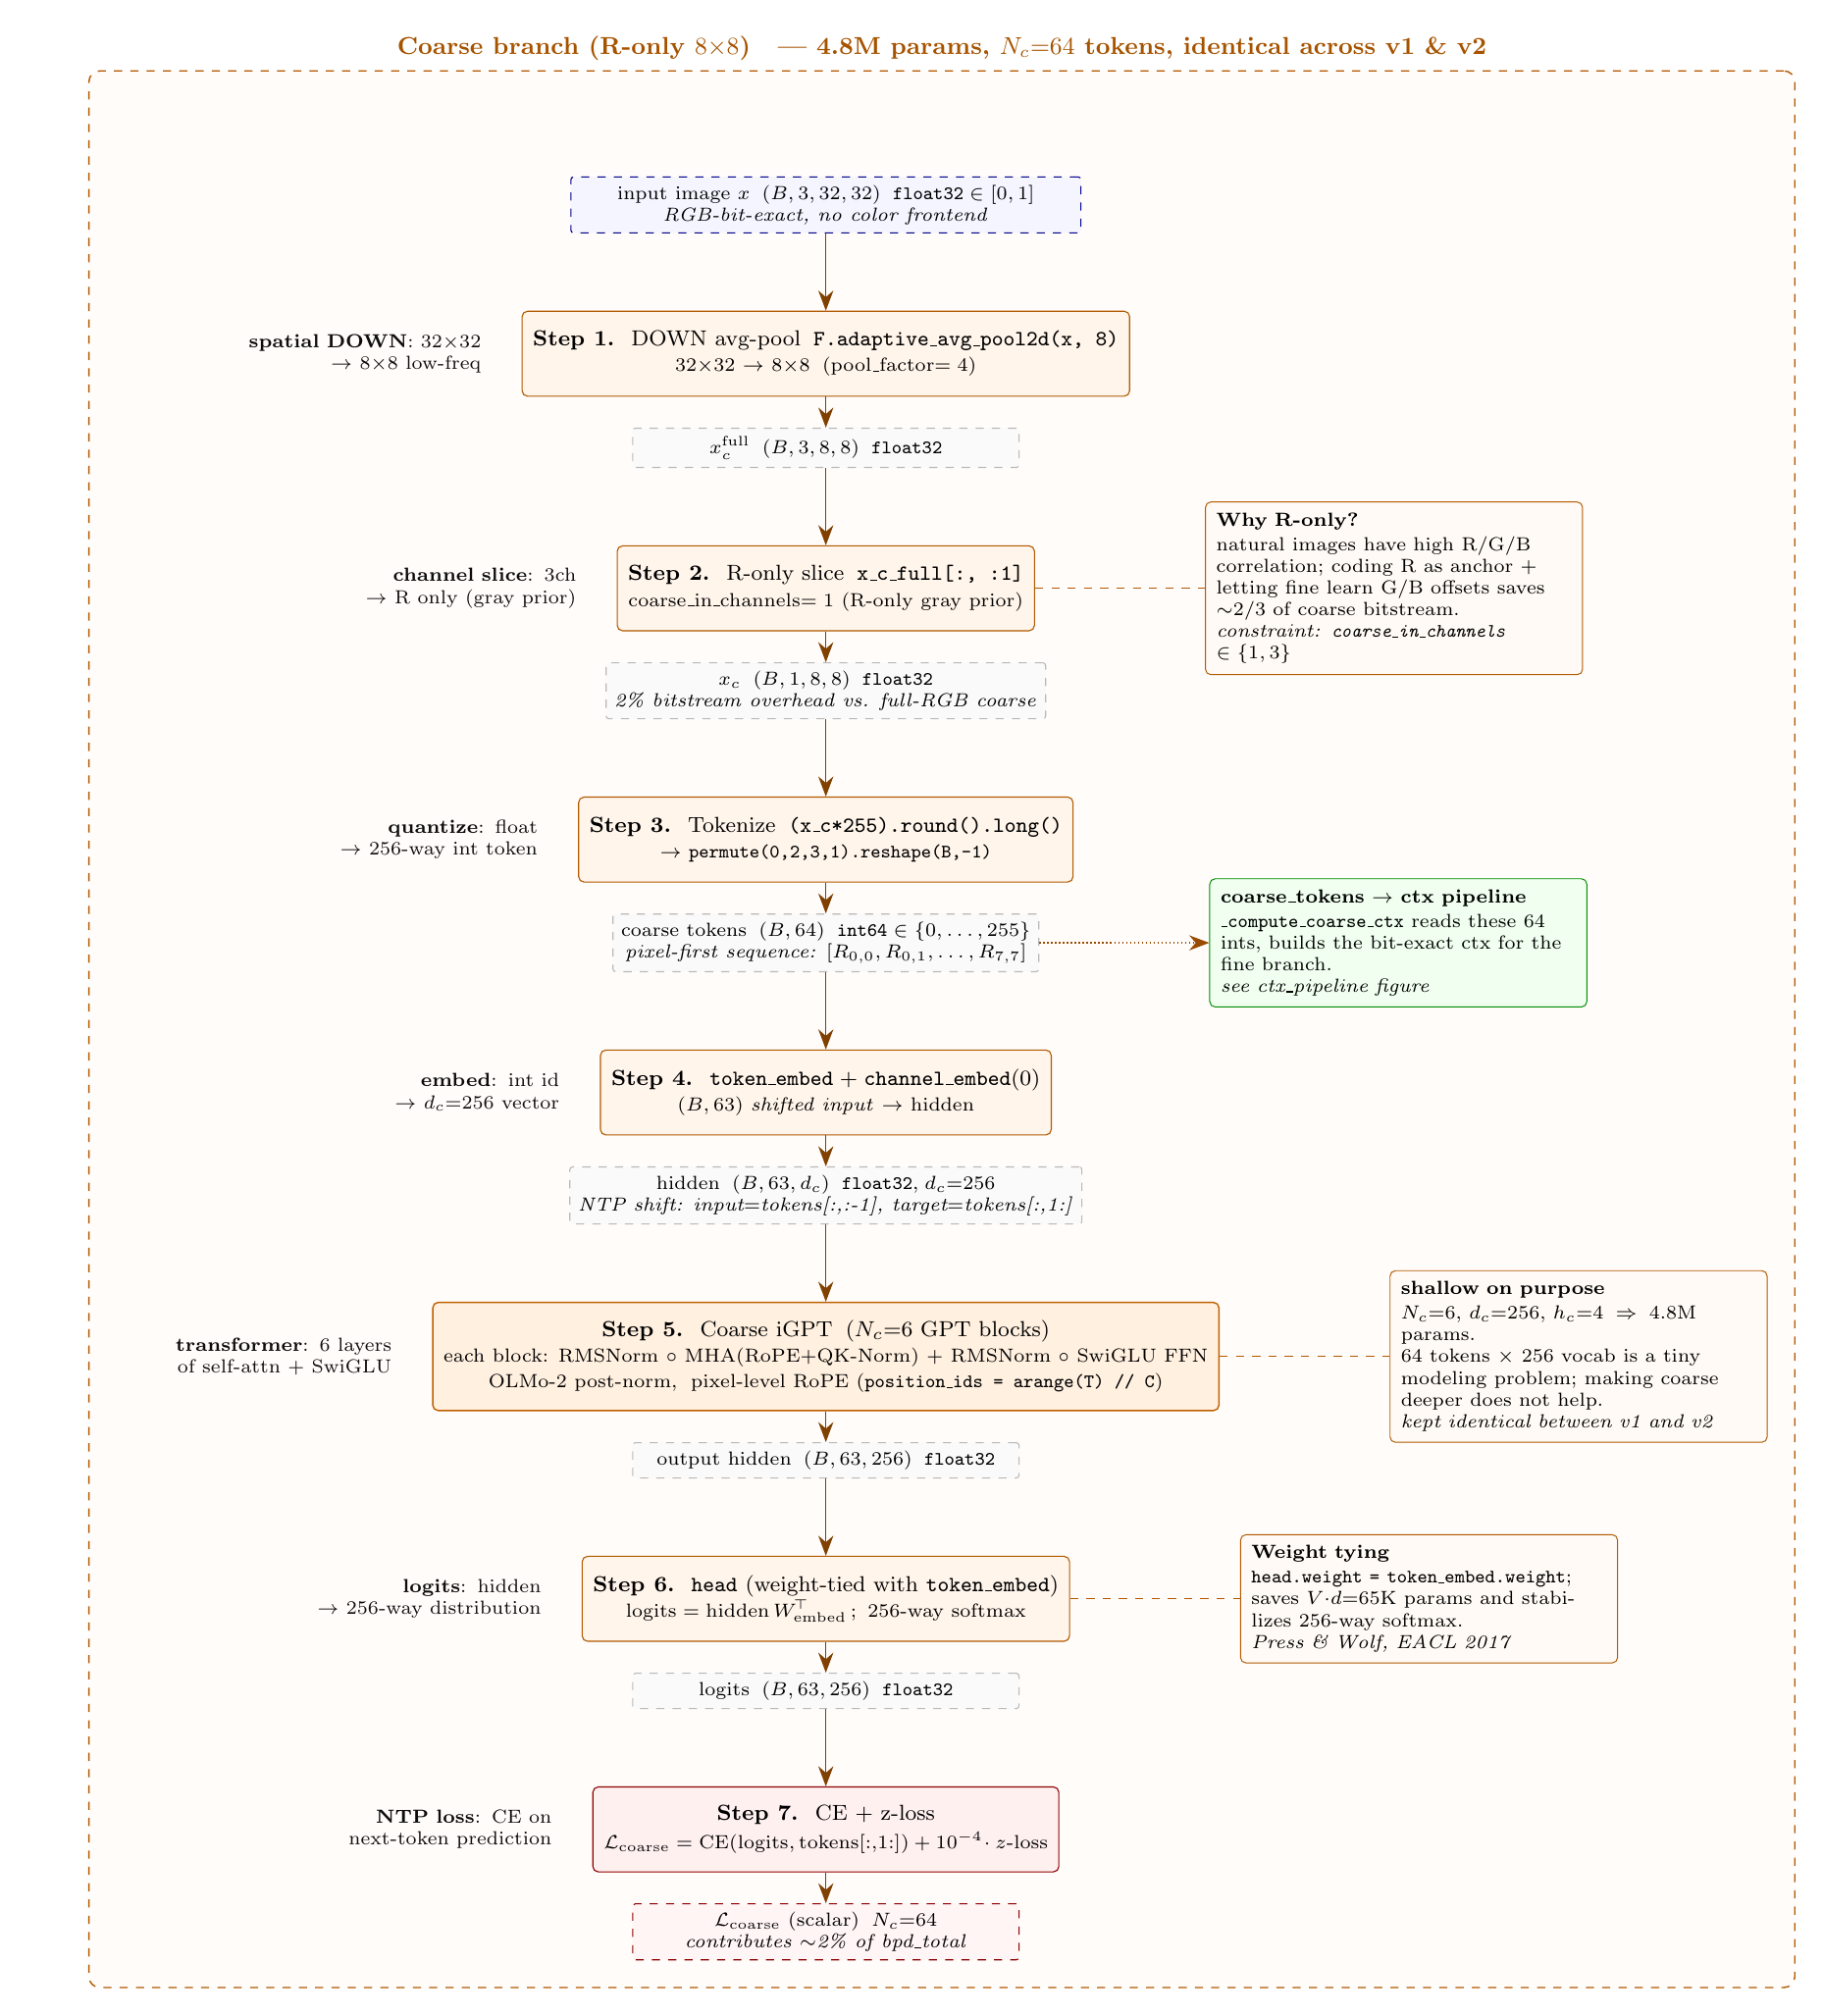
\begin{tikzpicture}[
    font=\footnotesize,
    >={Stealth[length=2.6mm]},
    node distance=10mm and 14mm,
    stepbox/.style ={draw, rounded corners=2pt, align=center,
                     minimum height=11mm, minimum width=50mm,
                     inner sep=4pt, fill=orange!8, draw=orange!70!black,
                     line width=0.4pt},
    blockbox/.style={draw, rounded corners=2pt, align=center,
                     minimum height=14mm, minimum width=50mm,
                     inner sep=4pt, fill=orange!12, draw=orange!75!black,
                     line width=0.5pt},
    tensor/.style  ={draw, dashed, rounded corners=1pt, align=center,
                     fill=gray!4, draw=gray!55, font=\scriptsize,
                     inner sep=3pt, minimum width=50mm},
    lossbox/.style ={draw, rounded corners=2pt, align=center,
                     minimum height=11mm, minimum width=50mm,
                     inner sep=4pt, fill=red!6, draw=red!55!black,
                     line width=0.4pt},
    callout/.style ={draw=orange!70!black, rounded corners=2pt,
                     fill=orange!4, align=left, font=\scriptsize,
                     inner sep=4pt, line width=0.35pt},
    flow/.style    ={->, line width=0.55pt, orange!50!black},
    sidearrow/.style={->, line width=0.45pt, orange!60!black, densely dotted},
]

% =========================================================
% TOP: invisible top spacer to host the fnbox label safely
% =========================================================
\node[minimum width=66mm, minimum height=8mm, inner sep=0pt]
     (topspacer) {};

% =========================================================
% TOP: input image
% =========================================================
\node[tensor, fill=blue!4, draw=blue!55!black, minimum width=66mm,
      below=2mm of topspacer]
     (xin) {input image $x$\;\;$(B,3,32,32)$\;\;\texttt{float32}\;$\in[0,1]$\\
            \textit{RGB-bit-exact, no color frontend}};

% =========================================================
% Step 1 -- DOWN avg-pool (RGB 32 -> 8)
% =========================================================
\node[stepbox, below=10mm of xin] (s1)
     {\textbf{Step 1.} \;DOWN avg-pool\;\;\texttt{F.adaptive\_avg\_pool2d(x, 8)}\\
      \scriptsize $32{\times}32$ $\to$ $8{\times}8$\;\;(pool\_factor$=4$)};
\node[tensor, below=4mm of s1] (t1)
     {$x_c^{\text{full}}$\;\;$(B,3,8,8)$\;\;\texttt{float32}};

% =========================================================
% Step 2 -- R-only channel slice
% =========================================================
\node[stepbox, below=10mm of t1] (s2)
     {\textbf{Step 2.} \;R-only slice\;\;\texttt{x\_c\_full[:, :1]}\\
      \scriptsize coarse\_in\_channels$=1$ (R-only gray prior)};
\node[tensor, below=4mm of s2] (t2)
     {$x_c$\;\;$(B,1,8,8)$\;\;\texttt{float32}\\
      \textit{2\% bitstream overhead vs. full-RGB coarse}};

% =========================================================
% Step 3 -- tokenize
% =========================================================
\node[stepbox, below=10mm of t2] (s3)
     {\textbf{Step 3.} \;Tokenize\;\;\texttt{(x\_c*255).round().long()}\\
      \scriptsize $\to$ \texttt{permute(0,2,3,1).reshape(B,-1)}};
\node[tensor, below=4mm of s3] (t3)
     {coarse tokens\;\;$(B,64)$\;\;\texttt{int64}\;$\in\{0,\dots,255\}$\\
      \textit{pixel-first sequence: $[R_{0,0}, R_{0,1}, \dots, R_{7,7}]$}};

% =========================================================
% Step 4 -- token_embed (256 -> d=256)
% =========================================================
\node[stepbox, below=10mm of t3] (s4)
     {\textbf{Step 4.} \;\texttt{token\_embed}\;+\;\texttt{channel\_embed}(0)\\
      \scriptsize $(B,63)$ \emph{shifted input} $\to$ hidden};
\node[tensor, below=4mm of s4] (t4)
     {hidden\;\;$(B,63,d_c)$\;\;\texttt{float32},\;$d_c{=}256$\\
      \textit{NTP shift: input$=$tokens[:,:-1], target$=$tokens[:,1:]}};

% =========================================================
% Step 5 -- coarse iGPT blocks (N_c = 6)
% =========================================================
\node[blockbox, below=10mm of t4] (s5)
     {\textbf{Step 5.} \;Coarse iGPT\;\;($N_c{=}6$ GPT blocks)\\
      \scriptsize each block: RMSNorm $\circ$ MHA(RoPE+QK-Norm) +
      RMSNorm $\circ$ SwiGLU FFN\\
      \scriptsize OLMo-2 post-norm,\; pixel-level RoPE
      (\texttt{position\_ids = arange(T) // C})};
\node[tensor, below=4mm of s5] (t5)
     {output hidden\;\;$(B,63,256)$\;\;\texttt{float32}};

% =========================================================
% Step 6 -- output head (weight-tied)
% =========================================================
\node[stepbox, below=10mm of t5] (s6)
     {\textbf{Step 6.} \;\texttt{head} (weight-tied with \texttt{token\_embed})\\
      \scriptsize $\text{logits} = \text{hidden}\,W^{\!\top}_{\text{embed}}$\,;\,
      256-way softmax};
\node[tensor, below=4mm of s6] (t6)
     {logits\;\;$(B,63,256)$\;\;\texttt{float32}};

% =========================================================
% Step 7 -- loss
% =========================================================
\node[lossbox, below=10mm of t6] (s7)
     {\textbf{Step 7.} \;CE + z-loss\\[1pt]
      \scriptsize $\mathcal{L}_{\text{coarse}} = \mathrm{CE}(\text{logits},
      \text{tokens[:,1:]}) + 10^{-4}\!\cdot z\text{-loss}$};
\node[tensor, below=4mm of s7, fill=red!4, draw=red!55!black]
     (out) {$\mathcal{L}_{\text{coarse}}$ (scalar)\;\;$N_c{=}64$\\
            \textit{contributes $\sim$2\% of bpd\_total}};

% =========================================================
% Side branch: coarse_tokens -> ctx pipeline
% =========================================================
\node[callout, right=22mm of t3, anchor=west, text width=46mm,
      fill=green!6, draw=green!55!black]
     (toctx) {\textbf{coarse\_tokens $\to$ ctx pipeline}\\[1pt]
              \texttt{\_compute\_coarse\_ctx} reads these 64 ints,
              builds the bit-exact ctx for the fine branch.\\
              \textit{see ctx\_pipeline figure}};
\draw[sidearrow] (t3.east) -- (toctx.west);

% =========================================================
% Right callouts
% =========================================================
\node[callout, right=22mm of s2, anchor=west, text width=46mm]
     (caR) {\textbf{Why R-only?}\\[1pt]
            natural images have high R/G/B correlation; coding R as
            anchor + letting fine learn G/B offsets saves $\sim$2/3
            of coarse bitstream.\\
            \textit{constraint: \texttt{coarse\_in\_channels} $\in \{1, 3\}$}};
\draw[orange!70!black, dashed, line width=0.35pt]
     (s2.east) -- (caR.west);

\node[callout, right=22mm of s5, anchor=west, text width=46mm]
     (caBlk) {\textbf{shallow on purpose}\\[1pt]
            $N_c{=}6$, $d_c{=}256$, $h_c{=}4$\;\;$\Rightarrow$\;\;4.8M params.\\
            64 tokens $\times$ 256 vocab is a tiny modeling problem;
            making coarse deeper does not help.\\
            \textit{kept identical between v1 and v2}};
\draw[orange!70!black, dashed, line width=0.35pt]
     (s5.east) -- (caBlk.west);

\node[callout, right=22mm of s6, anchor=west, text width=46mm]
     (caHead) {\textbf{Weight tying}\\[1pt]
            \texttt{head.weight = token\_embed.weight}; saves
            $V{\cdot}d{=}65$K params and stabilizes 256-way softmax.\\
            \textit{Press \& Wolf, EACL 2017}};
\draw[orange!70!black, dashed, line width=0.35pt]
     (s6.east) -- (caHead.west);

% =========================================================
% Left annotations
% =========================================================
\node[font=\scriptsize, gray!10!black, anchor=east, align=right,
      text width=46mm] (n1) at ($(s1.west)+(-4mm,0)$)
     {\textbf{spatial DOWN}: $32{\times}32$\\$\to$ $8{\times}8$ low-freq};
\node[font=\scriptsize, gray!10!black, anchor=east, align=right,
      text width=46mm] (n2) at ($(s2.west)+(-4mm,0)$)
     {\textbf{channel slice}: $3$ch\\$\to$ R only (gray prior)};
\node[font=\scriptsize, gray!10!black, anchor=east, align=right,
      text width=46mm] (n3) at ($(s3.west)+(-4mm,0)$)
     {\textbf{quantize}: float\\$\to$ 256-way int token};
\node[font=\scriptsize, gray!10!black, anchor=east, align=right,
      text width=46mm] (n4) at ($(s4.west)+(-4mm,0)$)
     {\textbf{embed}: int id\\$\to$ $d_c{=}256$ vector};
\node[font=\scriptsize, gray!10!black, anchor=east, align=right,
      text width=46mm] (n5) at ($(s5.west)+(-4mm,0)$)
     {\textbf{transformer}: 6 layers\\of self-attn + SwiGLU};
\node[font=\scriptsize, gray!10!black, anchor=east, align=right,
      text width=46mm] (n6) at ($(s6.west)+(-4mm,0)$)
     {\textbf{logits}: hidden\\$\to$ 256-way distribution};
\node[font=\scriptsize, gray!10!black, anchor=east, align=right,
      text width=46mm] (n7) at ($(s7.west)+(-4mm,0)$)
     {\textbf{NTP loss}: CE on\\next-token prediction};

% =========================================================
% Main flow arrows
% =========================================================
\draw[flow] (xin) -- (s1);
\draw[flow] (s1) -- (t1);
\draw[flow] (t1) -- (s2);
\draw[flow] (s2) -- (t2);
\draw[flow] (t2) -- (s3);
\draw[flow] (s3) -- (t3);
\draw[flow] (t3) -- (s4);
\draw[flow] (s4) -- (t4);
\draw[flow] (t4) -- (s5);
\draw[flow] (s5) -- (t5);
\draw[flow] (t5) -- (s6);
\draw[flow] (s6) -- (t6);
\draw[flow] (t6) -- (s7);
\draw[flow] (s7) -- (out);

% =========================================================
% Background frame
% =========================================================
\begin{pgfonlayer}{background}
  \node[draw=orange!70!black, dashed, rounded corners=4pt,
        fill=orange!2, line width=0.5pt, inner sep=10pt,
        fit=(topspacer)(s1)(s7)(t1)(out)(caR)(caBlk)(caHead)(toctx)(n1)(n7),
        label={[orange!65!black, font=\small\bfseries]above:%
              \textbf{Coarse branch (R-only $8{\times}8$)} \;
              --- 4.8M params, $N_c{=}64$ tokens, identical across v1 \& v2}]
        (cbox) {};
\end{pgfonlayer}

\end{tikzpicture}
\end{document}

%
% 配套 ctx_pipeline.tex / fine_pipeline.tex，把 coarse iGPT 分支 forward 全路径
% 在「张量 shape + dtype + 模块语义 + R-only 约束」三个层面具象化。
\documentclass[tikz,border=10pt]{standalone}
\usepackage{tikz}
\usepackage{amsmath,amssymb}
\usepackage{xcolor}
\usetikzlibrary{positioning,arrows.meta,calc,fit,backgrounds,shapes.geometric,
                decorations.pathreplacing,patterns}

\begin{document}
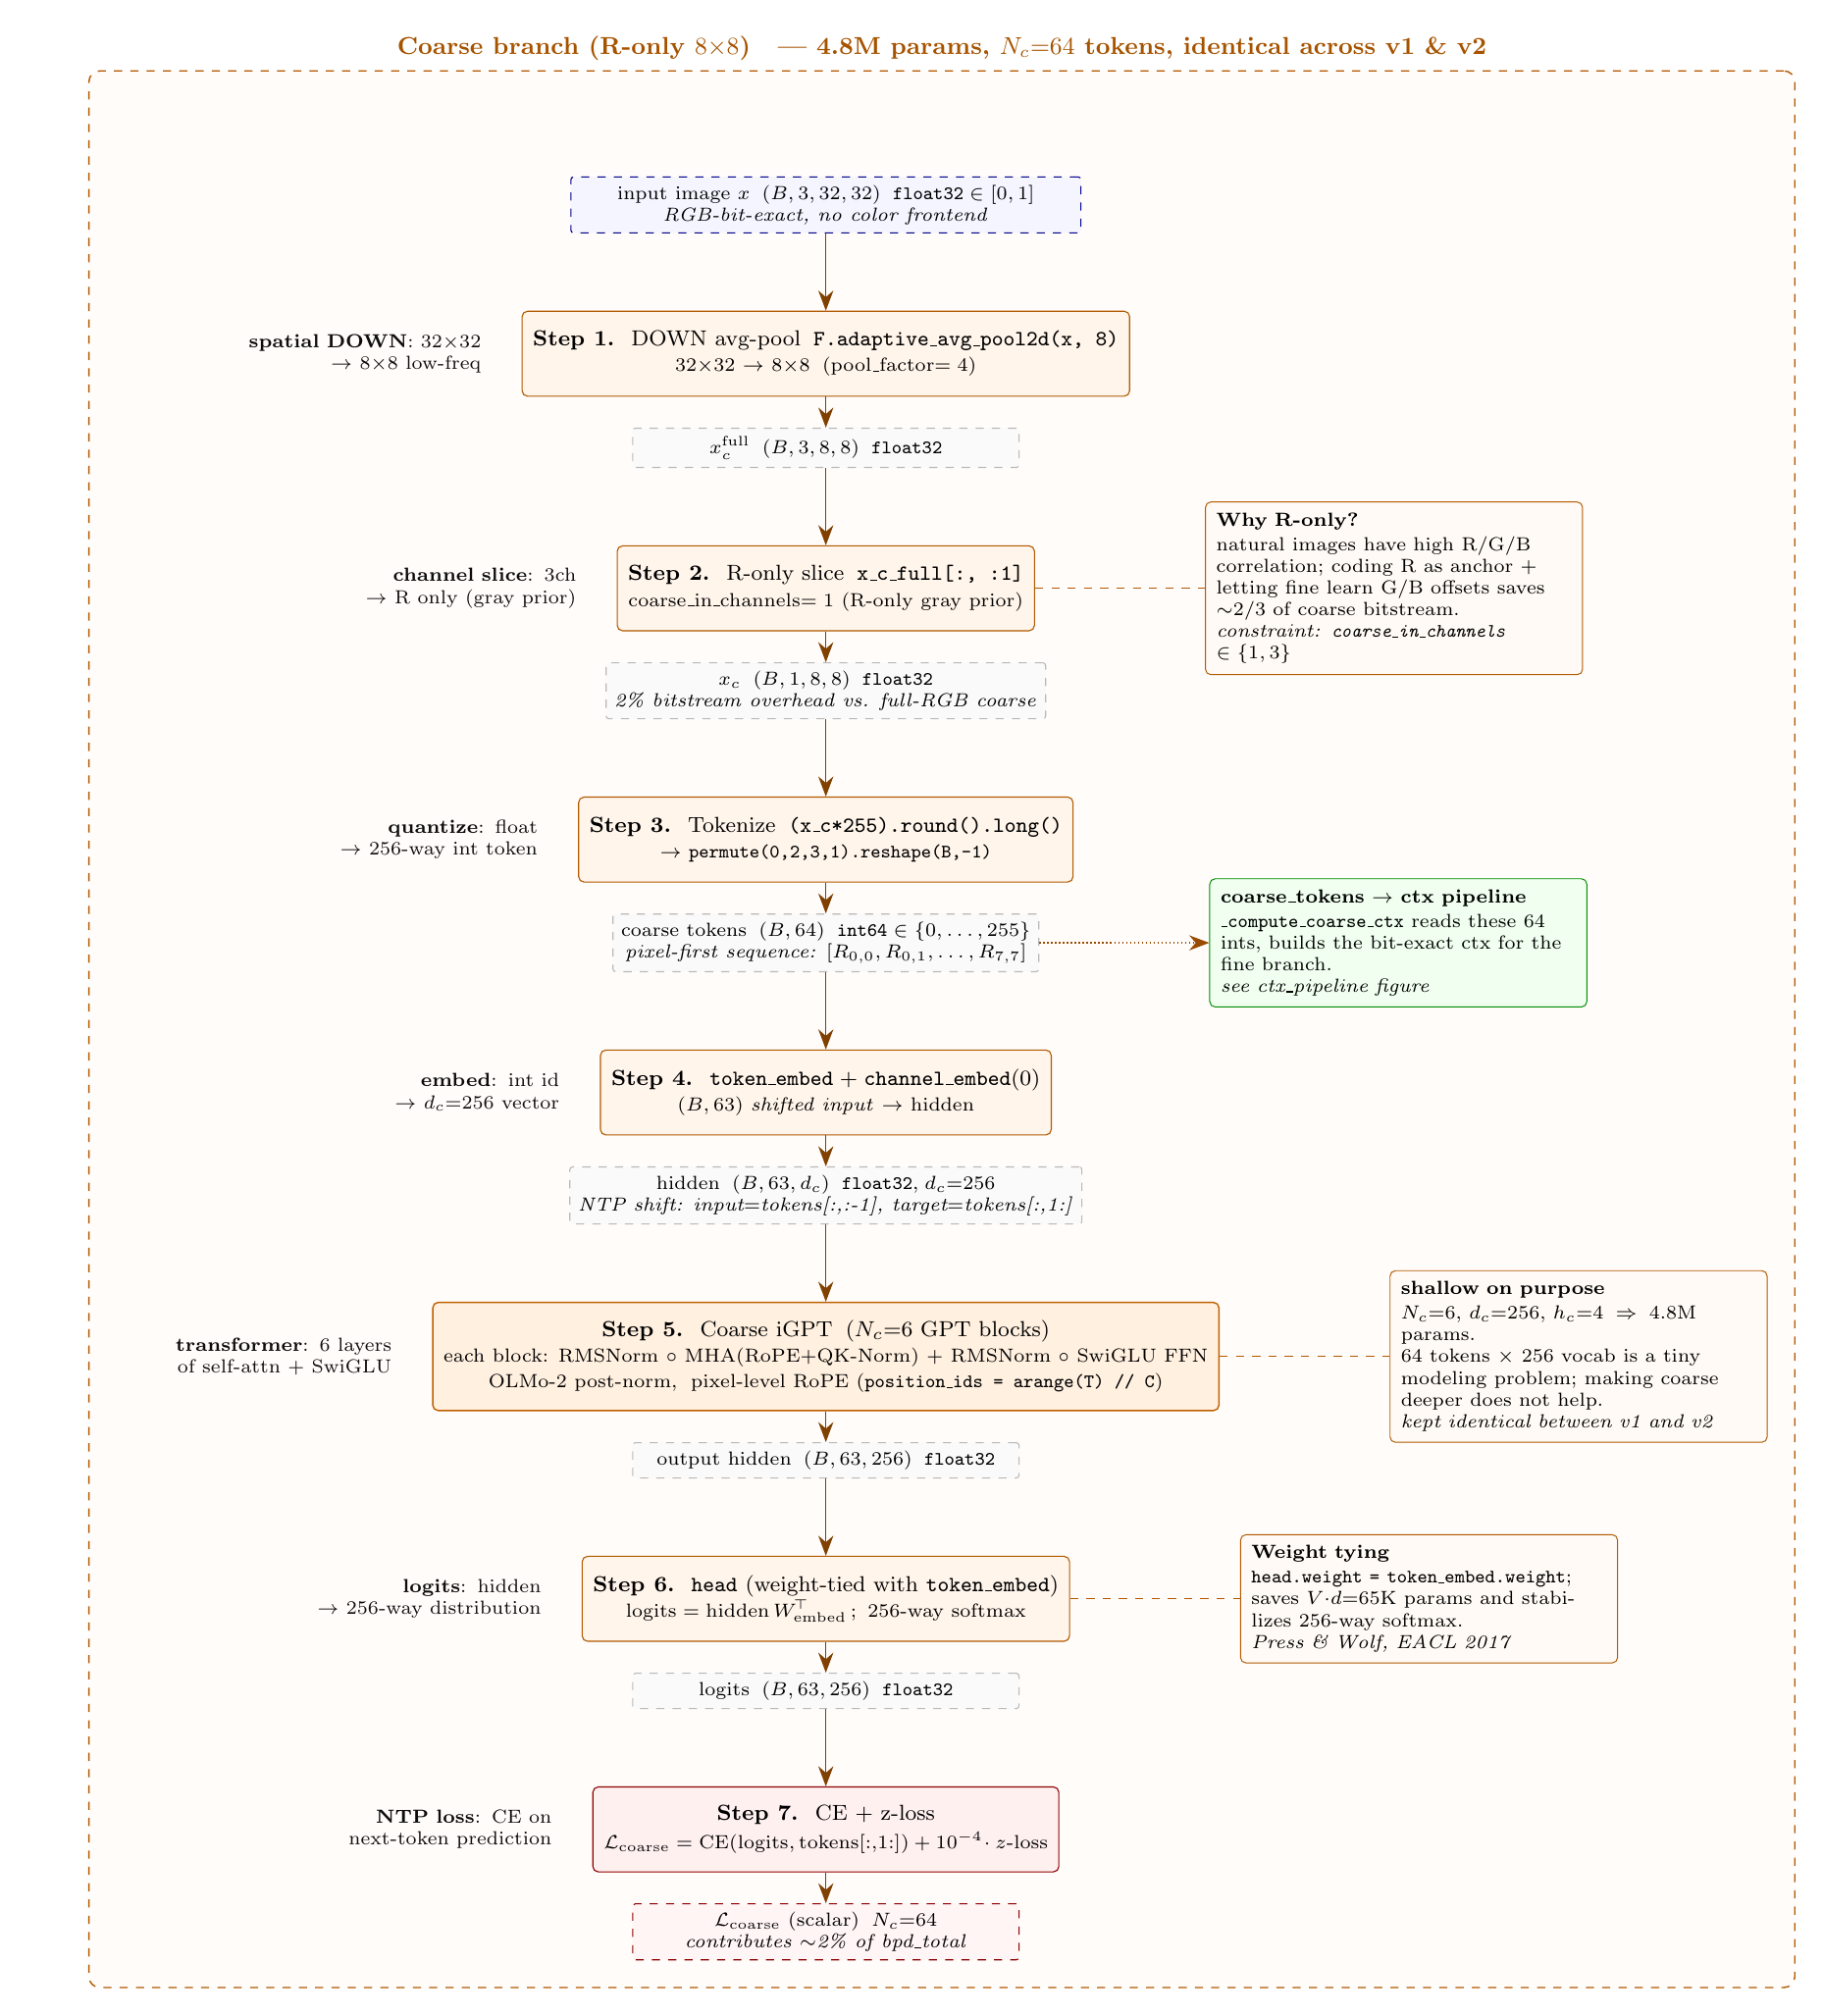
\begin{tikzpicture}[
    font=\footnotesize,
    >={Stealth[length=2.6mm]},
    node distance=10mm and 14mm,
    stepbox/.style ={draw, rounded corners=2pt, align=center,
                     minimum height=11mm, minimum width=50mm,
                     inner sep=4pt, fill=orange!8, draw=orange!70!black,
                     line width=0.4pt},
    blockbox/.style={draw, rounded corners=2pt, align=center,
                     minimum height=14mm, minimum width=50mm,
                     inner sep=4pt, fill=orange!12, draw=orange!75!black,
                     line width=0.5pt},
    tensor/.style  ={draw, dashed, rounded corners=1pt, align=center,
                     fill=gray!4, draw=gray!55, font=\scriptsize,
                     inner sep=3pt, minimum width=50mm},
    lossbox/.style ={draw, rounded corners=2pt, align=center,
                     minimum height=11mm, minimum width=50mm,
                     inner sep=4pt, fill=red!6, draw=red!55!black,
                     line width=0.4pt},
    callout/.style ={draw=orange!70!black, rounded corners=2pt,
                     fill=orange!4, align=left, font=\scriptsize,
                     inner sep=4pt, line width=0.35pt},
    flow/.style    ={->, line width=0.55pt, orange!50!black},
    sidearrow/.style={->, line width=0.45pt, orange!60!black, densely dotted},
]

% =========================================================
% TOP: invisible top spacer to host the fnbox label safely
% =========================================================
\node[minimum width=66mm, minimum height=8mm, inner sep=0pt]
     (topspacer) {};

% =========================================================
% TOP: input image
% =========================================================
\node[tensor, fill=blue!4, draw=blue!55!black, minimum width=66mm,
      below=2mm of topspacer]
     (xin) {input image $x$\;\;$(B,3,32,32)$\;\;\texttt{float32}\;$\in[0,1]$\\
            \textit{RGB-bit-exact, no color frontend}};

% =========================================================
% Step 1 -- DOWN avg-pool (RGB 32 -> 8)
% =========================================================
\node[stepbox, below=10mm of xin] (s1)
     {\textbf{Step 1.} \;DOWN avg-pool\;\;\texttt{F.adaptive\_avg\_pool2d(x, 8)}\\
      \scriptsize $32{\times}32$ $\to$ $8{\times}8$\;\;(pool\_factor$=4$)};
\node[tensor, below=4mm of s1] (t1)
     {$x_c^{\text{full}}$\;\;$(B,3,8,8)$\;\;\texttt{float32}};

% =========================================================
% Step 2 -- R-only channel slice
% =========================================================
\node[stepbox, below=10mm of t1] (s2)
     {\textbf{Step 2.} \;R-only slice\;\;\texttt{x\_c\_full[:, :1]}\\
      \scriptsize coarse\_in\_channels$=1$ (R-only gray prior)};
\node[tensor, below=4mm of s2] (t2)
     {$x_c$\;\;$(B,1,8,8)$\;\;\texttt{float32}\\
      \textit{2\% bitstream overhead vs. full-RGB coarse}};

% =========================================================
% Step 3 -- tokenize
% =========================================================
\node[stepbox, below=10mm of t2] (s3)
     {\textbf{Step 3.} \;Tokenize\;\;\texttt{(x\_c*255).round().long()}\\
      \scriptsize $\to$ \texttt{permute(0,2,3,1).reshape(B,-1)}};
\node[tensor, below=4mm of s3] (t3)
     {coarse tokens\;\;$(B,64)$\;\;\texttt{int64}\;$\in\{0,\dots,255\}$\\
      \textit{pixel-first sequence: $[R_{0,0}, R_{0,1}, \dots, R_{7,7}]$}};

% =========================================================
% Step 4 -- token_embed (256 -> d=256)
% =========================================================
\node[stepbox, below=10mm of t3] (s4)
     {\textbf{Step 4.} \;\texttt{token\_embed}\;+\;\texttt{channel\_embed}(0)\\
      \scriptsize $(B,63)$ \emph{shifted input} $\to$ hidden};
\node[tensor, below=4mm of s4] (t4)
     {hidden\;\;$(B,63,d_c)$\;\;\texttt{float32},\;$d_c{=}256$\\
      \textit{NTP shift: input$=$tokens[:,:-1], target$=$tokens[:,1:]}};

% =========================================================
% Step 5 -- coarse iGPT blocks (N_c = 6)
% =========================================================
\node[blockbox, below=10mm of t4] (s5)
     {\textbf{Step 5.} \;Coarse iGPT\;\;($N_c{=}6$ GPT blocks)\\
      \scriptsize each block: RMSNorm $\circ$ MHA(RoPE+QK-Norm) +
      RMSNorm $\circ$ SwiGLU FFN\\
      \scriptsize OLMo-2 post-norm,\; pixel-level RoPE
      (\texttt{position\_ids = arange(T) // C})};
\node[tensor, below=4mm of s5] (t5)
     {output hidden\;\;$(B,63,256)$\;\;\texttt{float32}};

% =========================================================
% Step 6 -- output head (weight-tied)
% =========================================================
\node[stepbox, below=10mm of t5] (s6)
     {\textbf{Step 6.} \;\texttt{head} (weight-tied with \texttt{token\_embed})\\
      \scriptsize $\text{logits} = \text{hidden}\,W^{\!\top}_{\text{embed}}$\,;\,
      256-way softmax};
\node[tensor, below=4mm of s6] (t6)
     {logits\;\;$(B,63,256)$\;\;\texttt{float32}};

% =========================================================
% Step 7 -- loss
% =========================================================
\node[lossbox, below=10mm of t6] (s7)
     {\textbf{Step 7.} \;CE + z-loss\\[1pt]
      \scriptsize $\mathcal{L}_{\text{coarse}} = \mathrm{CE}(\text{logits},
      \text{tokens[:,1:]}) + 10^{-4}\!\cdot z\text{-loss}$};
\node[tensor, below=4mm of s7, fill=red!4, draw=red!55!black]
     (out) {$\mathcal{L}_{\text{coarse}}$ (scalar)\;\;$N_c{=}64$\\
            \textit{contributes $\sim$2\% of bpd\_total}};

% =========================================================
% Side branch: coarse_tokens -> ctx pipeline
% =========================================================
\node[callout, right=22mm of t3, anchor=west, text width=46mm,
      fill=green!6, draw=green!55!black]
     (toctx) {\textbf{coarse\_tokens $\to$ ctx pipeline}\\[1pt]
              \texttt{\_compute\_coarse\_ctx} reads these 64 ints,
              builds the bit-exact ctx for the fine branch.\\
              \textit{see ctx\_pipeline figure}};
\draw[sidearrow] (t3.east) -- (toctx.west);

% =========================================================
% Right callouts
% =========================================================
\node[callout, right=22mm of s2, anchor=west, text width=46mm]
     (caR) {\textbf{Why R-only?}\\[1pt]
            natural images have high R/G/B correlation; coding R as
            anchor + letting fine learn G/B offsets saves $\sim$2/3
            of coarse bitstream.\\
            \textit{constraint: \texttt{coarse\_in\_channels} $\in \{1, 3\}$}};
\draw[orange!70!black, dashed, line width=0.35pt]
     (s2.east) -- (caR.west);

\node[callout, right=22mm of s5, anchor=west, text width=46mm]
     (caBlk) {\textbf{shallow on purpose}\\[1pt]
            $N_c{=}6$, $d_c{=}256$, $h_c{=}4$\;\;$\Rightarrow$\;\;4.8M params.\\
            64 tokens $\times$ 256 vocab is a tiny modeling problem;
            making coarse deeper does not help.\\
            \textit{kept identical between v1 and v2}};
\draw[orange!70!black, dashed, line width=0.35pt]
     (s5.east) -- (caBlk.west);

\node[callout, right=22mm of s6, anchor=west, text width=46mm]
     (caHead) {\textbf{Weight tying}\\[1pt]
            \texttt{head.weight = token\_embed.weight}; saves
            $V{\cdot}d{=}65$K params and stabilizes 256-way softmax.\\
            \textit{Press \& Wolf, EACL 2017}};
\draw[orange!70!black, dashed, line width=0.35pt]
     (s6.east) -- (caHead.west);

% =========================================================
% Left annotations
% =========================================================
\node[font=\scriptsize, gray!10!black, anchor=east, align=right,
      text width=46mm] (n1) at ($(s1.west)+(-4mm,0)$)
     {\textbf{spatial DOWN}: $32{\times}32$\\$\to$ $8{\times}8$ low-freq};
\node[font=\scriptsize, gray!10!black, anchor=east, align=right,
      text width=46mm] (n2) at ($(s2.west)+(-4mm,0)$)
     {\textbf{channel slice}: $3$ch\\$\to$ R only (gray prior)};
\node[font=\scriptsize, gray!10!black, anchor=east, align=right,
      text width=46mm] (n3) at ($(s3.west)+(-4mm,0)$)
     {\textbf{quantize}: float\\$\to$ 256-way int token};
\node[font=\scriptsize, gray!10!black, anchor=east, align=right,
      text width=46mm] (n4) at ($(s4.west)+(-4mm,0)$)
     {\textbf{embed}: int id\\$\to$ $d_c{=}256$ vector};
\node[font=\scriptsize, gray!10!black, anchor=east, align=right,
      text width=46mm] (n5) at ($(s5.west)+(-4mm,0)$)
     {\textbf{transformer}: 6 layers\\of self-attn + SwiGLU};
\node[font=\scriptsize, gray!10!black, anchor=east, align=right,
      text width=46mm] (n6) at ($(s6.west)+(-4mm,0)$)
     {\textbf{logits}: hidden\\$\to$ 256-way distribution};
\node[font=\scriptsize, gray!10!black, anchor=east, align=right,
      text width=46mm] (n7) at ($(s7.west)+(-4mm,0)$)
     {\textbf{NTP loss}: CE on\\next-token prediction};

% =========================================================
% Main flow arrows
% =========================================================
\draw[flow] (xin) -- (s1);
\draw[flow] (s1) -- (t1);
\draw[flow] (t1) -- (s2);
\draw[flow] (s2) -- (t2);
\draw[flow] (t2) -- (s3);
\draw[flow] (s3) -- (t3);
\draw[flow] (t3) -- (s4);
\draw[flow] (s4) -- (t4);
\draw[flow] (t4) -- (s5);
\draw[flow] (s5) -- (t5);
\draw[flow] (t5) -- (s6);
\draw[flow] (s6) -- (t6);
\draw[flow] (t6) -- (s7);
\draw[flow] (s7) -- (out);

% =========================================================
% Background frame
% =========================================================
\begin{pgfonlayer}{background}
  \node[draw=orange!70!black, dashed, rounded corners=4pt,
        fill=orange!2, line width=0.5pt, inner sep=10pt,
        fit=(topspacer)(s1)(s7)(t1)(out)(caR)(caBlk)(caHead)(toctx)(n1)(n7),
        label={[orange!65!black, font=\small\bfseries]above:%
              \textbf{Coarse branch (R-only $8{\times}8$)} \;
              --- 4.8M params, $N_c{=}64$ tokens, identical across v1 \& v2}]
        (cbox) {};
\end{pgfonlayer}

\end{tikzpicture}
\end{document}

%
% 配套 ctx_pipeline.tex / fine_pipeline.tex，把 coarse iGPT 分支 forward 全路径
% 在「张量 shape + dtype + 模块语义 + R-only 约束」三个层面具象化。
\documentclass[tikz,border=10pt]{standalone}
\usepackage{tikz}
\usepackage{amsmath,amssymb}
\usepackage{xcolor}
\usetikzlibrary{positioning,arrows.meta,calc,fit,backgrounds,shapes.geometric,
                decorations.pathreplacing,patterns}

\begin{document}
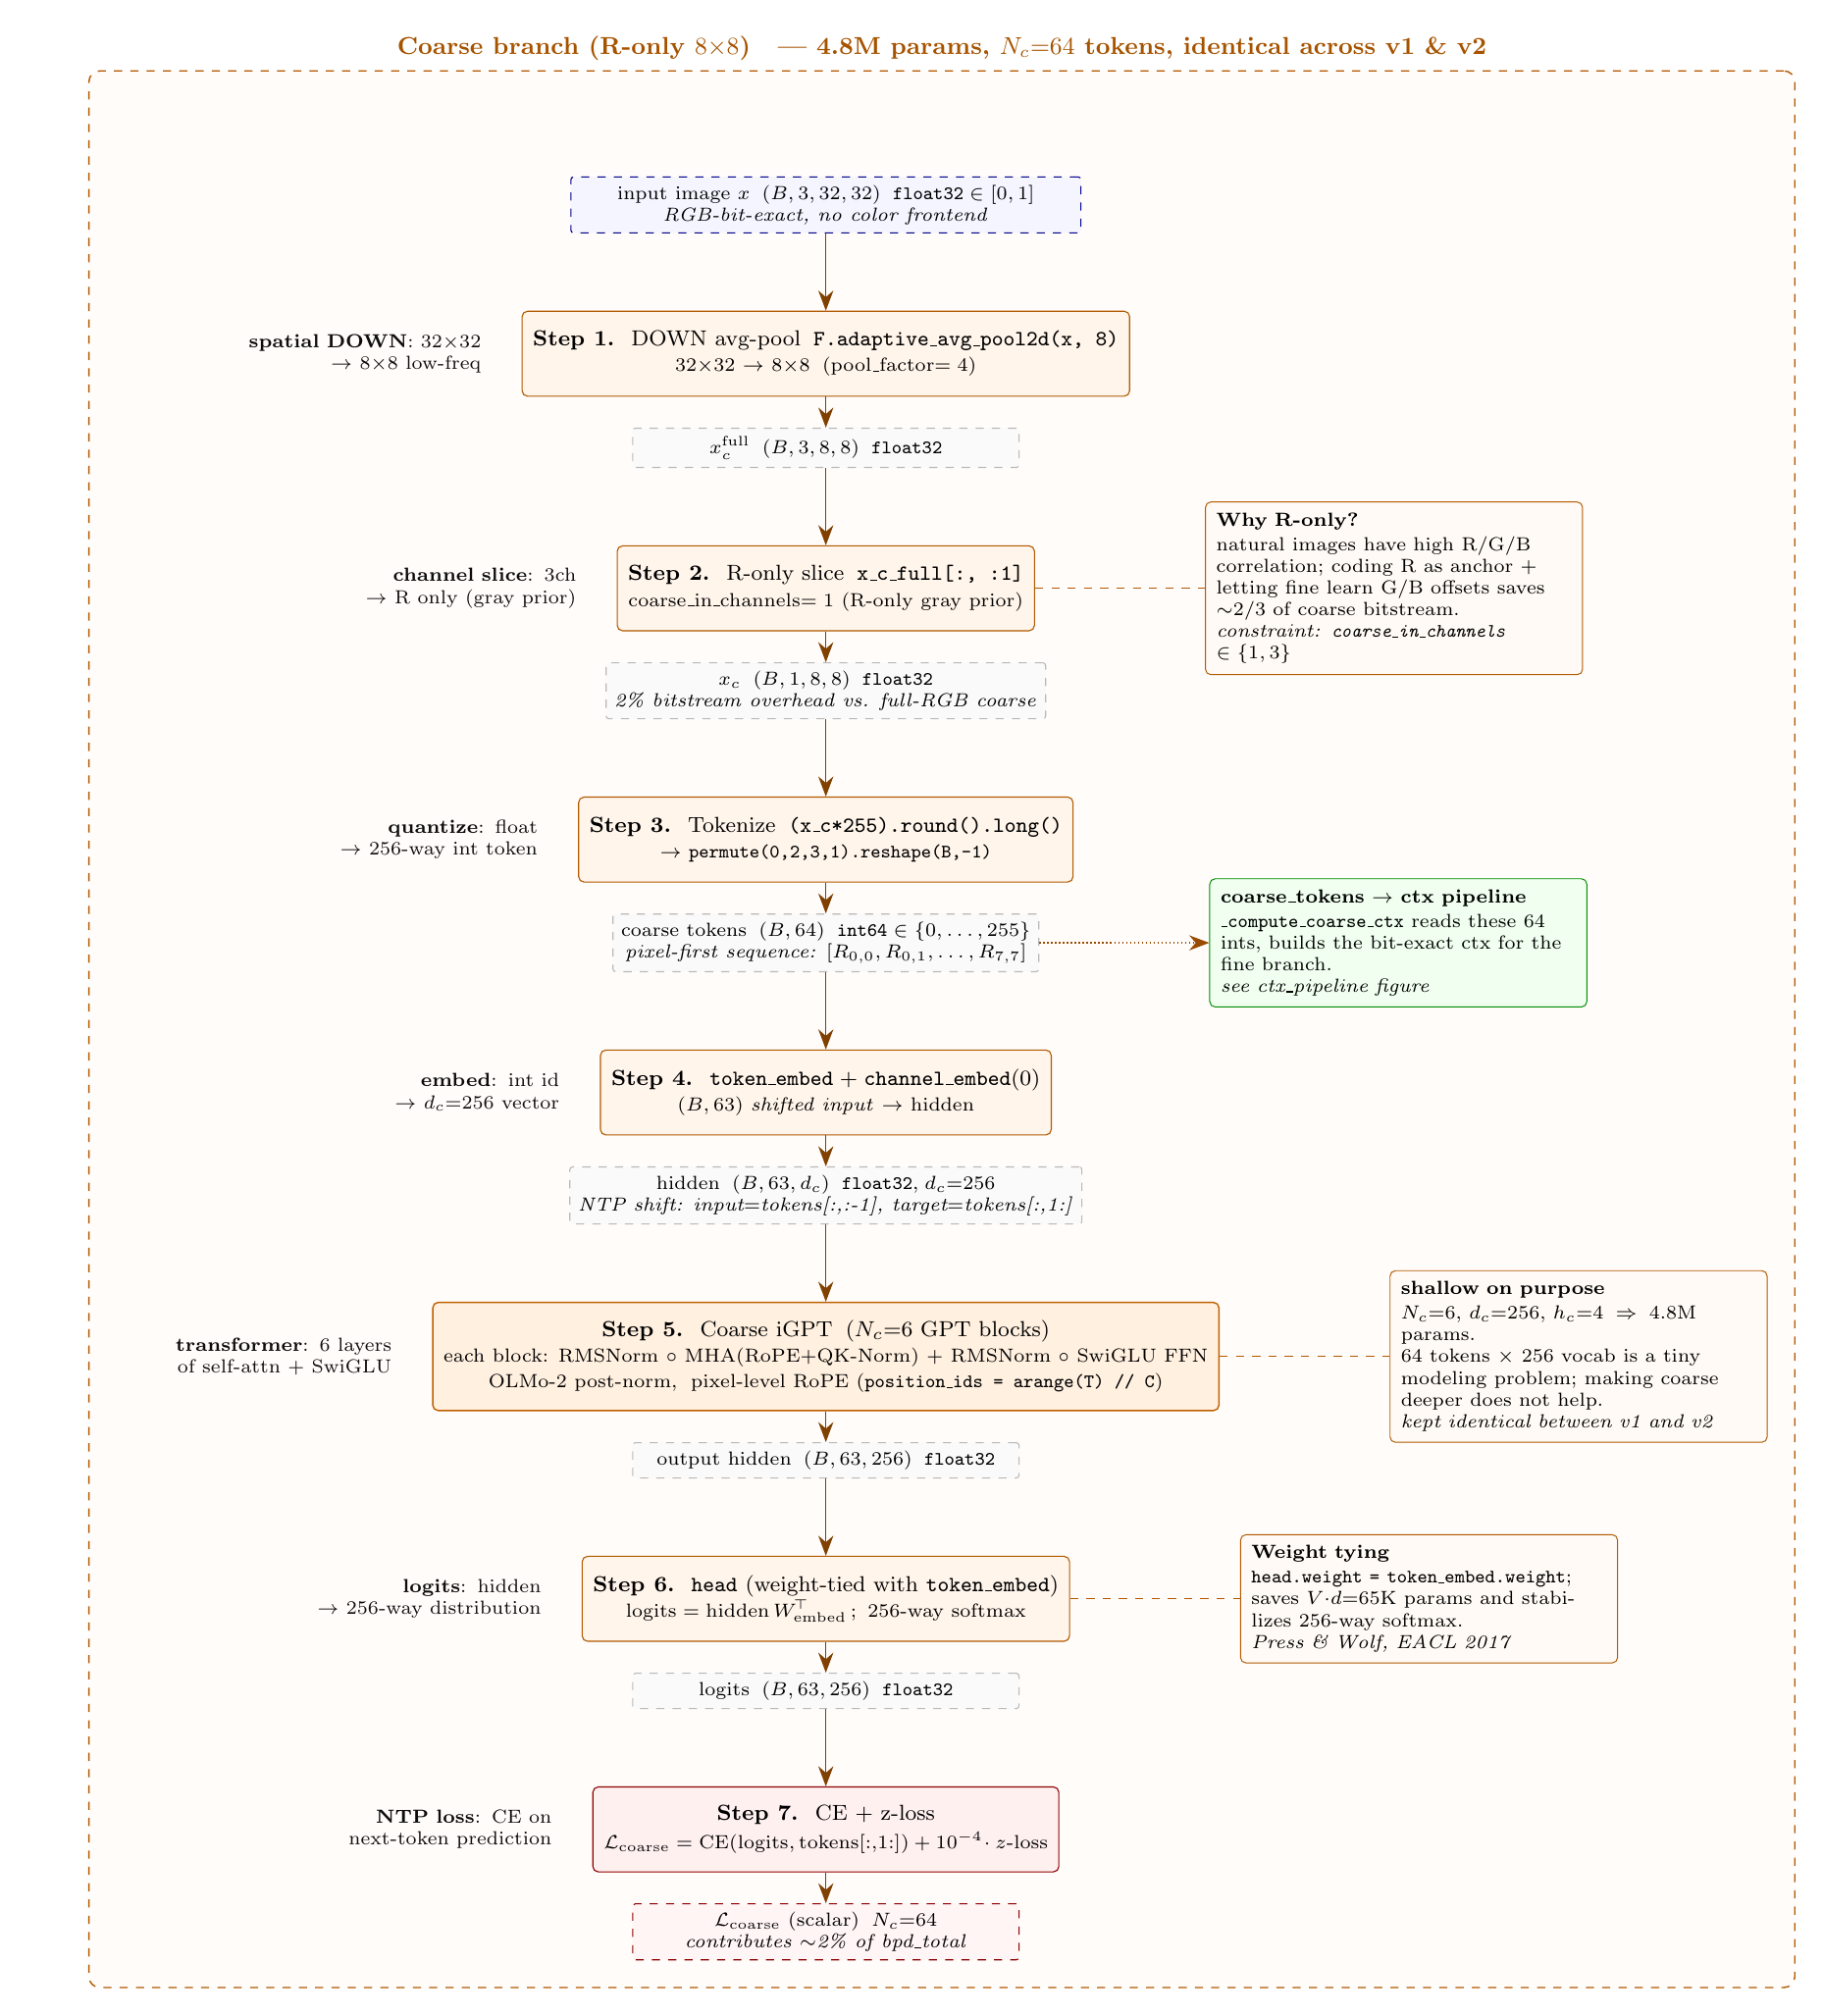
\begin{tikzpicture}[
    font=\footnotesize,
    >={Stealth[length=2.6mm]},
    node distance=10mm and 14mm,
    stepbox/.style ={draw, rounded corners=2pt, align=center,
                     minimum height=11mm, minimum width=50mm,
                     inner sep=4pt, fill=orange!8, draw=orange!70!black,
                     line width=0.4pt},
    blockbox/.style={draw, rounded corners=2pt, align=center,
                     minimum height=14mm, minimum width=50mm,
                     inner sep=4pt, fill=orange!12, draw=orange!75!black,
                     line width=0.5pt},
    tensor/.style  ={draw, dashed, rounded corners=1pt, align=center,
                     fill=gray!4, draw=gray!55, font=\scriptsize,
                     inner sep=3pt, minimum width=50mm},
    lossbox/.style ={draw, rounded corners=2pt, align=center,
                     minimum height=11mm, minimum width=50mm,
                     inner sep=4pt, fill=red!6, draw=red!55!black,
                     line width=0.4pt},
    callout/.style ={draw=orange!70!black, rounded corners=2pt,
                     fill=orange!4, align=left, font=\scriptsize,
                     inner sep=4pt, line width=0.35pt},
    flow/.style    ={->, line width=0.55pt, orange!50!black},
    sidearrow/.style={->, line width=0.45pt, orange!60!black, densely dotted},
]

% =========================================================
% TOP: invisible top spacer to host the fnbox label safely
% =========================================================
\node[minimum width=66mm, minimum height=8mm, inner sep=0pt]
     (topspacer) {};

% =========================================================
% TOP: input image
% =========================================================
\node[tensor, fill=blue!4, draw=blue!55!black, minimum width=66mm,
      below=2mm of topspacer]
     (xin) {input image $x$\;\;$(B,3,32,32)$\;\;\texttt{float32}\;$\in[0,1]$\\
            \textit{RGB-bit-exact, no color frontend}};

% =========================================================
% Step 1 -- DOWN avg-pool (RGB 32 -> 8)
% =========================================================
\node[stepbox, below=10mm of xin] (s1)
     {\textbf{Step 1.} \;DOWN avg-pool\;\;\texttt{F.adaptive\_avg\_pool2d(x, 8)}\\
      \scriptsize $32{\times}32$ $\to$ $8{\times}8$\;\;(pool\_factor$=4$)};
\node[tensor, below=4mm of s1] (t1)
     {$x_c^{\text{full}}$\;\;$(B,3,8,8)$\;\;\texttt{float32}};

% =========================================================
% Step 2 -- R-only channel slice
% =========================================================
\node[stepbox, below=10mm of t1] (s2)
     {\textbf{Step 2.} \;R-only slice\;\;\texttt{x\_c\_full[:, :1]}\\
      \scriptsize coarse\_in\_channels$=1$ (R-only gray prior)};
\node[tensor, below=4mm of s2] (t2)
     {$x_c$\;\;$(B,1,8,8)$\;\;\texttt{float32}\\
      \textit{2\% bitstream overhead vs. full-RGB coarse}};

% =========================================================
% Step 3 -- tokenize
% =========================================================
\node[stepbox, below=10mm of t2] (s3)
     {\textbf{Step 3.} \;Tokenize\;\;\texttt{(x\_c*255).round().long()}\\
      \scriptsize $\to$ \texttt{permute(0,2,3,1).reshape(B,-1)}};
\node[tensor, below=4mm of s3] (t3)
     {coarse tokens\;\;$(B,64)$\;\;\texttt{int64}\;$\in\{0,\dots,255\}$\\
      \textit{pixel-first sequence: $[R_{0,0}, R_{0,1}, \dots, R_{7,7}]$}};

% =========================================================
% Step 4 -- token_embed (256 -> d=256)
% =========================================================
\node[stepbox, below=10mm of t3] (s4)
     {\textbf{Step 4.} \;\texttt{token\_embed}\;+\;\texttt{channel\_embed}(0)\\
      \scriptsize $(B,63)$ \emph{shifted input} $\to$ hidden};
\node[tensor, below=4mm of s4] (t4)
     {hidden\;\;$(B,63,d_c)$\;\;\texttt{float32},\;$d_c{=}256$\\
      \textit{NTP shift: input$=$tokens[:,:-1], target$=$tokens[:,1:]}};

% =========================================================
% Step 5 -- coarse iGPT blocks (N_c = 6)
% =========================================================
\node[blockbox, below=10mm of t4] (s5)
     {\textbf{Step 5.} \;Coarse iGPT\;\;($N_c{=}6$ GPT blocks)\\
      \scriptsize each block: RMSNorm $\circ$ MHA(RoPE+QK-Norm) +
      RMSNorm $\circ$ SwiGLU FFN\\
      \scriptsize OLMo-2 post-norm,\; pixel-level RoPE
      (\texttt{position\_ids = arange(T) // C})};
\node[tensor, below=4mm of s5] (t5)
     {output hidden\;\;$(B,63,256)$\;\;\texttt{float32}};

% =========================================================
% Step 6 -- output head (weight-tied)
% =========================================================
\node[stepbox, below=10mm of t5] (s6)
     {\textbf{Step 6.} \;\texttt{head} (weight-tied with \texttt{token\_embed})\\
      \scriptsize $\text{logits} = \text{hidden}\,W^{\!\top}_{\text{embed}}$\,;\,
      256-way softmax};
\node[tensor, below=4mm of s6] (t6)
     {logits\;\;$(B,63,256)$\;\;\texttt{float32}};

% =========================================================
% Step 7 -- loss
% =========================================================
\node[lossbox, below=10mm of t6] (s7)
     {\textbf{Step 7.} \;CE + z-loss\\[1pt]
      \scriptsize $\mathcal{L}_{\text{coarse}} = \mathrm{CE}(\text{logits},
      \text{tokens[:,1:]}) + 10^{-4}\!\cdot z\text{-loss}$};
\node[tensor, below=4mm of s7, fill=red!4, draw=red!55!black]
     (out) {$\mathcal{L}_{\text{coarse}}$ (scalar)\;\;$N_c{=}64$\\
            \textit{contributes $\sim$2\% of bpd\_total}};

% =========================================================
% Side branch: coarse_tokens -> ctx pipeline
% =========================================================
\node[callout, right=22mm of t3, anchor=west, text width=46mm,
      fill=green!6, draw=green!55!black]
     (toctx) {\textbf{coarse\_tokens $\to$ ctx pipeline}\\[1pt]
              \texttt{\_compute\_coarse\_ctx} reads these 64 ints,
              builds the bit-exact ctx for the fine branch.\\
              \textit{see ctx\_pipeline figure}};
\draw[sidearrow] (t3.east) -- (toctx.west);

% =========================================================
% Right callouts
% =========================================================
\node[callout, right=22mm of s2, anchor=west, text width=46mm]
     (caR) {\textbf{Why R-only?}\\[1pt]
            natural images have high R/G/B correlation; coding R as
            anchor + letting fine learn G/B offsets saves $\sim$2/3
            of coarse bitstream.\\
            \textit{constraint: \texttt{coarse\_in\_channels} $\in \{1, 3\}$}};
\draw[orange!70!black, dashed, line width=0.35pt]
     (s2.east) -- (caR.west);

\node[callout, right=22mm of s5, anchor=west, text width=46mm]
     (caBlk) {\textbf{shallow on purpose}\\[1pt]
            $N_c{=}6$, $d_c{=}256$, $h_c{=}4$\;\;$\Rightarrow$\;\;4.8M params.\\
            64 tokens $\times$ 256 vocab is a tiny modeling problem;
            making coarse deeper does not help.\\
            \textit{kept identical between v1 and v2}};
\draw[orange!70!black, dashed, line width=0.35pt]
     (s5.east) -- (caBlk.west);

\node[callout, right=22mm of s6, anchor=west, text width=46mm]
     (caHead) {\textbf{Weight tying}\\[1pt]
            \texttt{head.weight = token\_embed.weight}; saves
            $V{\cdot}d{=}65$K params and stabilizes 256-way softmax.\\
            \textit{Press \& Wolf, EACL 2017}};
\draw[orange!70!black, dashed, line width=0.35pt]
     (s6.east) -- (caHead.west);

% =========================================================
% Left annotations
% =========================================================
\node[font=\scriptsize, gray!10!black, anchor=east, align=right,
      text width=46mm] (n1) at ($(s1.west)+(-4mm,0)$)
     {\textbf{spatial DOWN}: $32{\times}32$\\$\to$ $8{\times}8$ low-freq};
\node[font=\scriptsize, gray!10!black, anchor=east, align=right,
      text width=46mm] (n2) at ($(s2.west)+(-4mm,0)$)
     {\textbf{channel slice}: $3$ch\\$\to$ R only (gray prior)};
\node[font=\scriptsize, gray!10!black, anchor=east, align=right,
      text width=46mm] (n3) at ($(s3.west)+(-4mm,0)$)
     {\textbf{quantize}: float\\$\to$ 256-way int token};
\node[font=\scriptsize, gray!10!black, anchor=east, align=right,
      text width=46mm] (n4) at ($(s4.west)+(-4mm,0)$)
     {\textbf{embed}: int id\\$\to$ $d_c{=}256$ vector};
\node[font=\scriptsize, gray!10!black, anchor=east, align=right,
      text width=46mm] (n5) at ($(s5.west)+(-4mm,0)$)
     {\textbf{transformer}: 6 layers\\of self-attn + SwiGLU};
\node[font=\scriptsize, gray!10!black, anchor=east, align=right,
      text width=46mm] (n6) at ($(s6.west)+(-4mm,0)$)
     {\textbf{logits}: hidden\\$\to$ 256-way distribution};
\node[font=\scriptsize, gray!10!black, anchor=east, align=right,
      text width=46mm] (n7) at ($(s7.west)+(-4mm,0)$)
     {\textbf{NTP loss}: CE on\\next-token prediction};

% =========================================================
% Main flow arrows
% =========================================================
\draw[flow] (xin) -- (s1);
\draw[flow] (s1) -- (t1);
\draw[flow] (t1) -- (s2);
\draw[flow] (s2) -- (t2);
\draw[flow] (t2) -- (s3);
\draw[flow] (s3) -- (t3);
\draw[flow] (t3) -- (s4);
\draw[flow] (s4) -- (t4);
\draw[flow] (t4) -- (s5);
\draw[flow] (s5) -- (t5);
\draw[flow] (t5) -- (s6);
\draw[flow] (s6) -- (t6);
\draw[flow] (t6) -- (s7);
\draw[flow] (s7) -- (out);

% =========================================================
% Background frame
% =========================================================
\begin{pgfonlayer}{background}
  \node[draw=orange!70!black, dashed, rounded corners=4pt,
        fill=orange!2, line width=0.5pt, inner sep=10pt,
        fit=(topspacer)(s1)(s7)(t1)(out)(caR)(caBlk)(caHead)(toctx)(n1)(n7),
        label={[orange!65!black, font=\small\bfseries]above:%
              \textbf{Coarse branch (R-only $8{\times}8$)} \;
              --- 4.8M params, $N_c{=}64$ tokens, identical across v1 \& v2}]
        (cbox) {};
\end{pgfonlayer}

\end{tikzpicture}
\end{document}

%
% 配套 ctx_pipeline.tex / fine_pipeline.tex，把 coarse iGPT 分支 forward 全路径
% 在「张量 shape + dtype + 模块语义 + R-only 约束」三个层面具象化。
\documentclass[tikz,border=10pt]{standalone}
\usepackage{tikz}
\usepackage{amsmath,amssymb}
\usepackage{xcolor}
\usetikzlibrary{positioning,arrows.meta,calc,fit,backgrounds,shapes.geometric,
                decorations.pathreplacing,patterns}

\begin{document}
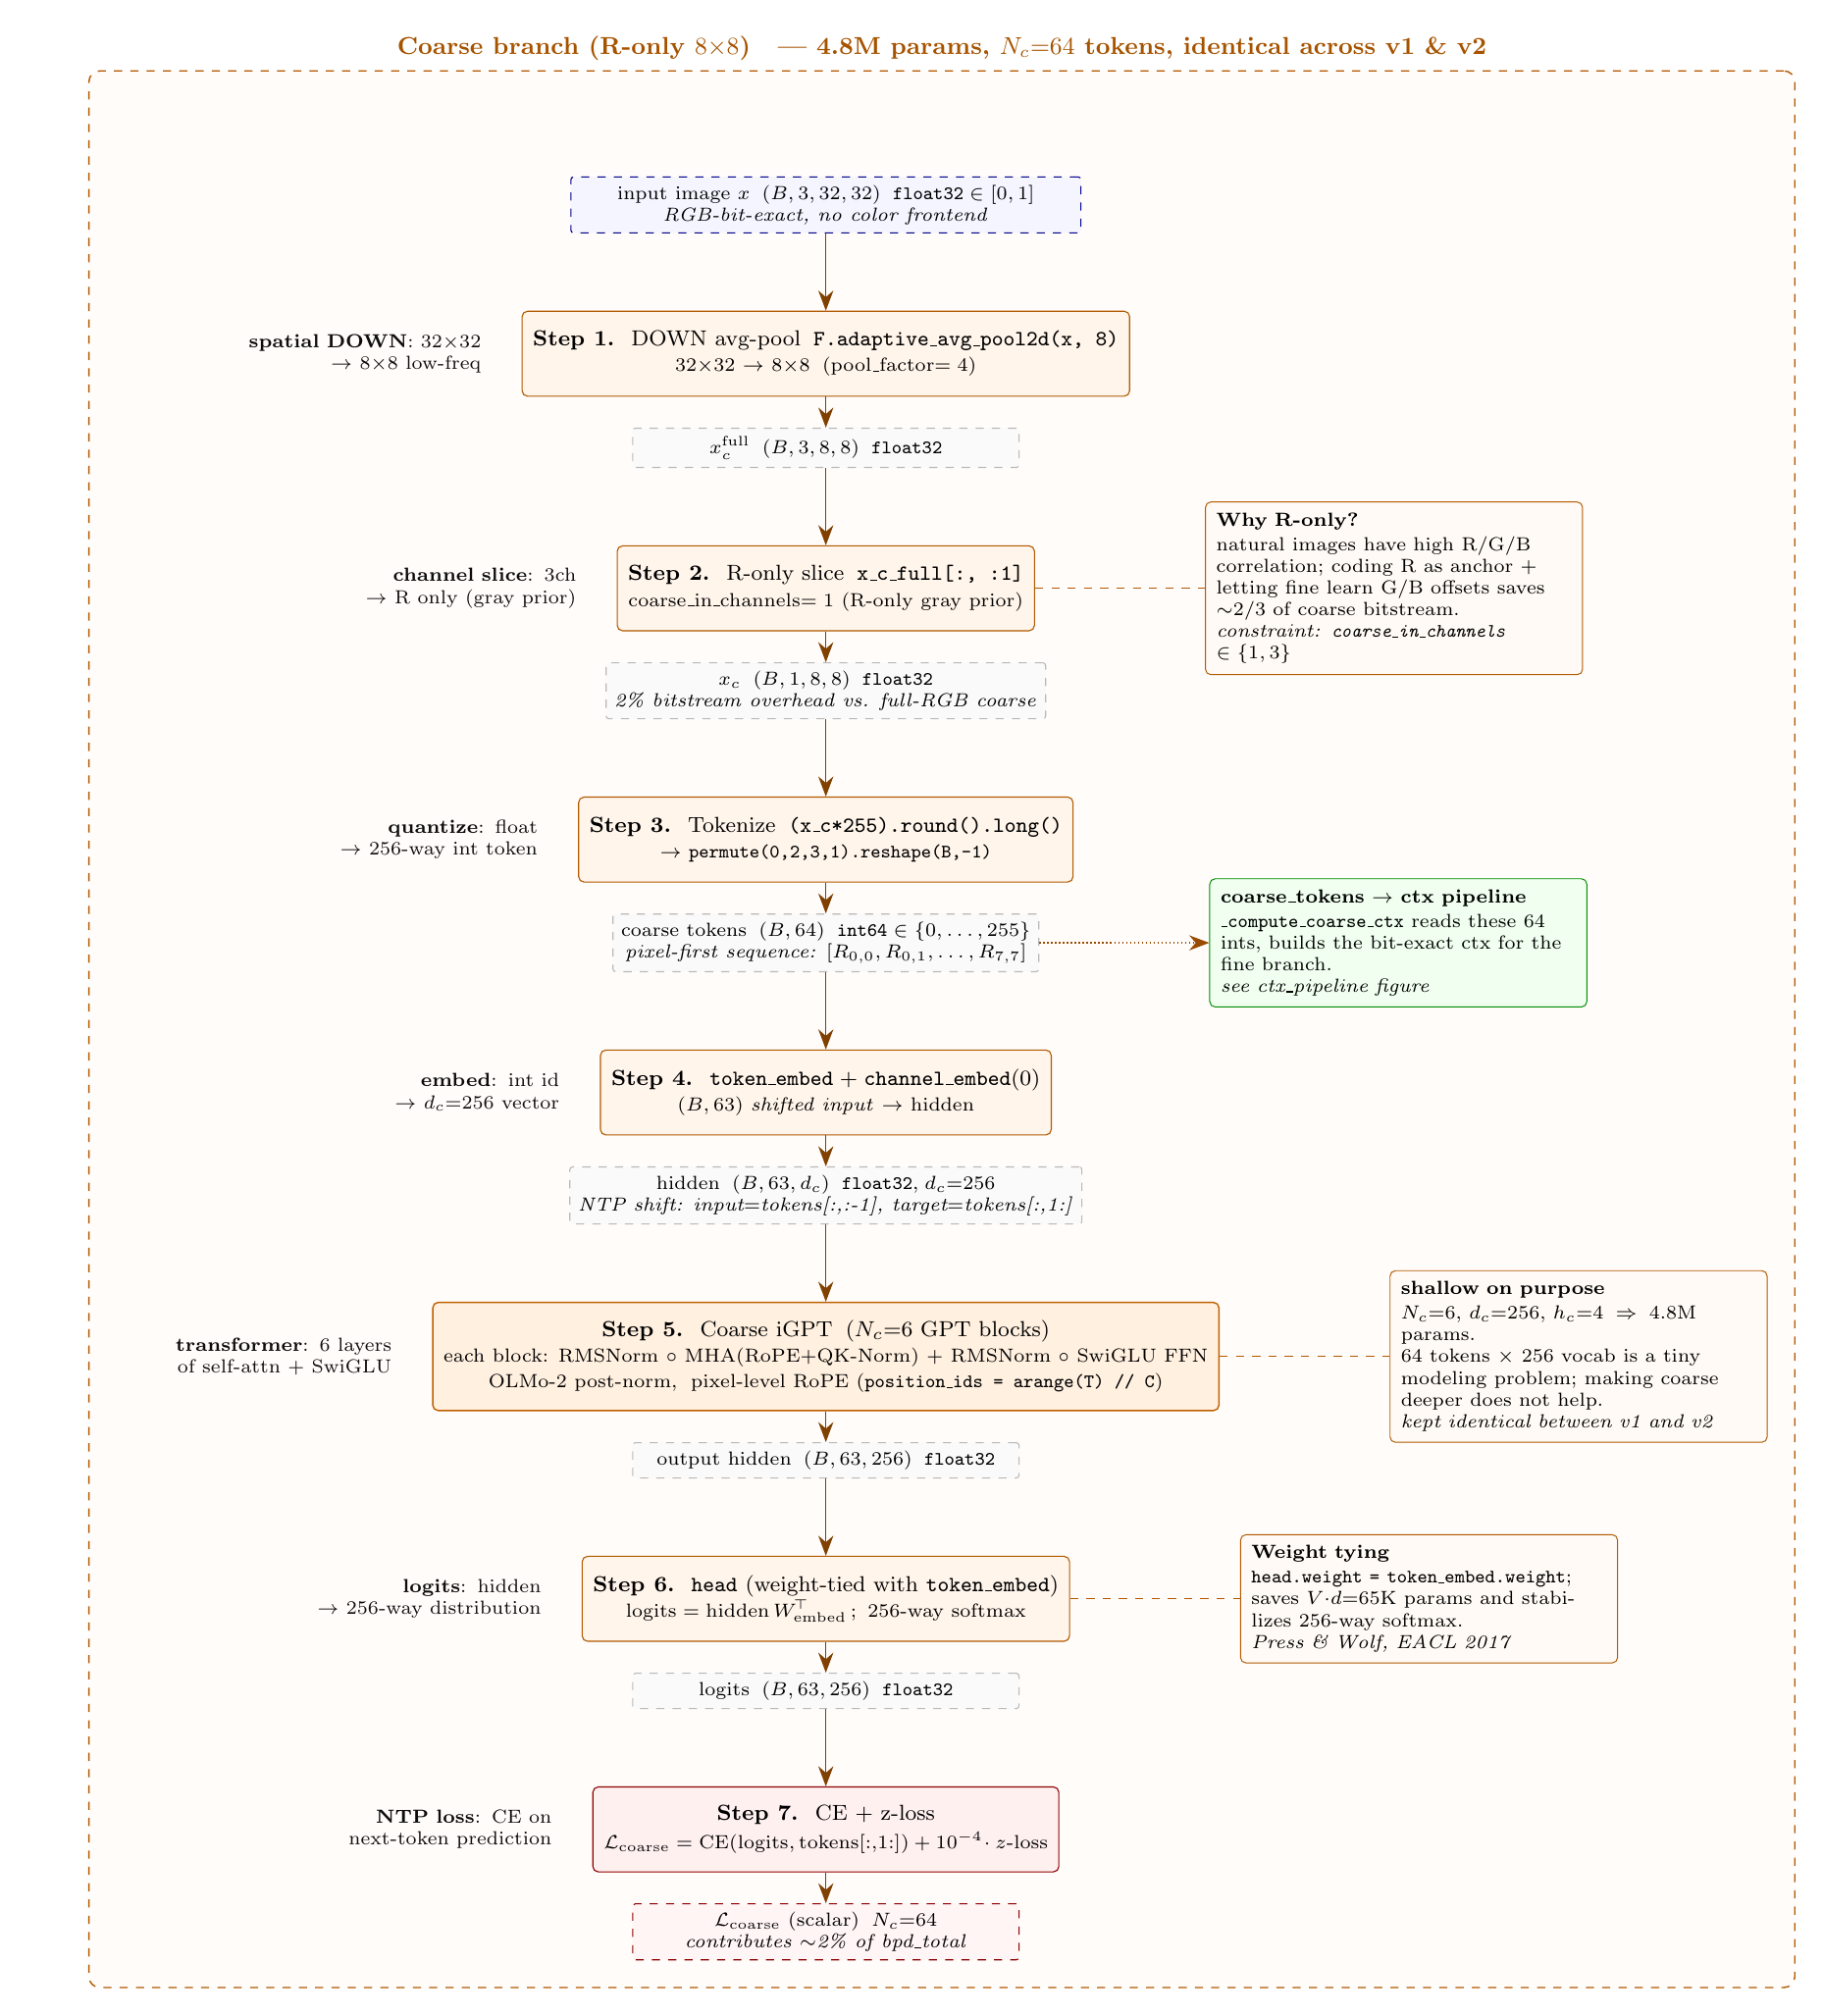
\begin{tikzpicture}[
    font=\footnotesize,
    >={Stealth[length=2.6mm]},
    node distance=10mm and 14mm,
    stepbox/.style ={draw, rounded corners=2pt, align=center,
                     minimum height=11mm, minimum width=50mm,
                     inner sep=4pt, fill=orange!8, draw=orange!70!black,
                     line width=0.4pt},
    blockbox/.style={draw, rounded corners=2pt, align=center,
                     minimum height=14mm, minimum width=50mm,
                     inner sep=4pt, fill=orange!12, draw=orange!75!black,
                     line width=0.5pt},
    tensor/.style  ={draw, dashed, rounded corners=1pt, align=center,
                     fill=gray!4, draw=gray!55, font=\scriptsize,
                     inner sep=3pt, minimum width=50mm},
    lossbox/.style ={draw, rounded corners=2pt, align=center,
                     minimum height=11mm, minimum width=50mm,
                     inner sep=4pt, fill=red!6, draw=red!55!black,
                     line width=0.4pt},
    callout/.style ={draw=orange!70!black, rounded corners=2pt,
                     fill=orange!4, align=left, font=\scriptsize,
                     inner sep=4pt, line width=0.35pt},
    flow/.style    ={->, line width=0.55pt, orange!50!black},
    sidearrow/.style={->, line width=0.45pt, orange!60!black, densely dotted},
]

% =========================================================
% TOP: invisible top spacer to host the fnbox label safely
% =========================================================
\node[minimum width=66mm, minimum height=8mm, inner sep=0pt]
     (topspacer) {};

% =========================================================
% TOP: input image
% =========================================================
\node[tensor, fill=blue!4, draw=blue!55!black, minimum width=66mm,
      below=2mm of topspacer]
     (xin) {input image $x$\;\;$(B,3,32,32)$\;\;\texttt{float32}\;$\in[0,1]$\\
            \textit{RGB-bit-exact, no color frontend}};

% =========================================================
% Step 1 -- DOWN avg-pool (RGB 32 -> 8)
% =========================================================
\node[stepbox, below=10mm of xin] (s1)
     {\textbf{Step 1.} \;DOWN avg-pool\;\;\texttt{F.adaptive\_avg\_pool2d(x, 8)}\\
      \scriptsize $32{\times}32$ $\to$ $8{\times}8$\;\;(pool\_factor$=4$)};
\node[tensor, below=4mm of s1] (t1)
     {$x_c^{\text{full}}$\;\;$(B,3,8,8)$\;\;\texttt{float32}};

% =========================================================
% Step 2 -- R-only channel slice
% =========================================================
\node[stepbox, below=10mm of t1] (s2)
     {\textbf{Step 2.} \;R-only slice\;\;\texttt{x\_c\_full[:, :1]}\\
      \scriptsize coarse\_in\_channels$=1$ (R-only gray prior)};
\node[tensor, below=4mm of s2] (t2)
     {$x_c$\;\;$(B,1,8,8)$\;\;\texttt{float32}\\
      \textit{2\% bitstream overhead vs. full-RGB coarse}};

% =========================================================
% Step 3 -- tokenize
% =========================================================
\node[stepbox, below=10mm of t2] (s3)
     {\textbf{Step 3.} \;Tokenize\;\;\texttt{(x\_c*255).round().long()}\\
      \scriptsize $\to$ \texttt{permute(0,2,3,1).reshape(B,-1)}};
\node[tensor, below=4mm of s3] (t3)
     {coarse tokens\;\;$(B,64)$\;\;\texttt{int64}\;$\in\{0,\dots,255\}$\\
      \textit{pixel-first sequence: $[R_{0,0}, R_{0,1}, \dots, R_{7,7}]$}};

% =========================================================
% Step 4 -- token_embed (256 -> d=256)
% =========================================================
\node[stepbox, below=10mm of t3] (s4)
     {\textbf{Step 4.} \;\texttt{token\_embed}\;+\;\texttt{channel\_embed}(0)\\
      \scriptsize $(B,63)$ \emph{shifted input} $\to$ hidden};
\node[tensor, below=4mm of s4] (t4)
     {hidden\;\;$(B,63,d_c)$\;\;\texttt{float32},\;$d_c{=}256$\\
      \textit{NTP shift: input$=$tokens[:,:-1], target$=$tokens[:,1:]}};

% =========================================================
% Step 5 -- coarse iGPT blocks (N_c = 6)
% =========================================================
\node[blockbox, below=10mm of t4] (s5)
     {\textbf{Step 5.} \;Coarse iGPT\;\;($N_c{=}6$ GPT blocks)\\
      \scriptsize each block: RMSNorm $\circ$ MHA(RoPE+QK-Norm) +
      RMSNorm $\circ$ SwiGLU FFN\\
      \scriptsize OLMo-2 post-norm,\; pixel-level RoPE
      (\texttt{position\_ids = arange(T) // C})};
\node[tensor, below=4mm of s5] (t5)
     {output hidden\;\;$(B,63,256)$\;\;\texttt{float32}};

% =========================================================
% Step 6 -- output head (weight-tied)
% =========================================================
\node[stepbox, below=10mm of t5] (s6)
     {\textbf{Step 6.} \;\texttt{head} (weight-tied with \texttt{token\_embed})\\
      \scriptsize $\text{logits} = \text{hidden}\,W^{\!\top}_{\text{embed}}$\,;\,
      256-way softmax};
\node[tensor, below=4mm of s6] (t6)
     {logits\;\;$(B,63,256)$\;\;\texttt{float32}};

% =========================================================
% Step 7 -- loss
% =========================================================
\node[lossbox, below=10mm of t6] (s7)
     {\textbf{Step 7.} \;CE + z-loss\\[1pt]
      \scriptsize $\mathcal{L}_{\text{coarse}} = \mathrm{CE}(\text{logits},
      \text{tokens[:,1:]}) + 10^{-4}\!\cdot z\text{-loss}$};
\node[tensor, below=4mm of s7, fill=red!4, draw=red!55!black]
     (out) {$\mathcal{L}_{\text{coarse}}$ (scalar)\;\;$N_c{=}64$\\
            \textit{contributes $\sim$2\% of bpd\_total}};

% =========================================================
% Side branch: coarse_tokens -> ctx pipeline
% =========================================================
\node[callout, right=22mm of t3, anchor=west, text width=46mm,
      fill=green!6, draw=green!55!black]
     (toctx) {\textbf{coarse\_tokens $\to$ ctx pipeline}\\[1pt]
              \texttt{\_compute\_coarse\_ctx} reads these 64 ints,
              builds the bit-exact ctx for the fine branch.\\
              \textit{see ctx\_pipeline figure}};
\draw[sidearrow] (t3.east) -- (toctx.west);

% =========================================================
% Right callouts
% =========================================================
\node[callout, right=22mm of s2, anchor=west, text width=46mm]
     (caR) {\textbf{Why R-only?}\\[1pt]
            natural images have high R/G/B correlation; coding R as
            anchor + letting fine learn G/B offsets saves $\sim$2/3
            of coarse bitstream.\\
            \textit{constraint: \texttt{coarse\_in\_channels} $\in \{1, 3\}$}};
\draw[orange!70!black, dashed, line width=0.35pt]
     (s2.east) -- (caR.west);

\node[callout, right=22mm of s5, anchor=west, text width=46mm]
     (caBlk) {\textbf{shallow on purpose}\\[1pt]
            $N_c{=}6$, $d_c{=}256$, $h_c{=}4$\;\;$\Rightarrow$\;\;4.8M params.\\
            64 tokens $\times$ 256 vocab is a tiny modeling problem;
            making coarse deeper does not help.\\
            \textit{kept identical between v1 and v2}};
\draw[orange!70!black, dashed, line width=0.35pt]
     (s5.east) -- (caBlk.west);

\node[callout, right=22mm of s6, anchor=west, text width=46mm]
     (caHead) {\textbf{Weight tying}\\[1pt]
            \texttt{head.weight = token\_embed.weight}; saves
            $V{\cdot}d{=}65$K params and stabilizes 256-way softmax.\\
            \textit{Press \& Wolf, EACL 2017}};
\draw[orange!70!black, dashed, line width=0.35pt]
     (s6.east) -- (caHead.west);

% =========================================================
% Left annotations
% =========================================================
\node[font=\scriptsize, gray!10!black, anchor=east, align=right,
      text width=46mm] (n1) at ($(s1.west)+(-4mm,0)$)
     {\textbf{spatial DOWN}: $32{\times}32$\\$\to$ $8{\times}8$ low-freq};
\node[font=\scriptsize, gray!10!black, anchor=east, align=right,
      text width=46mm] (n2) at ($(s2.west)+(-4mm,0)$)
     {\textbf{channel slice}: $3$ch\\$\to$ R only (gray prior)};
\node[font=\scriptsize, gray!10!black, anchor=east, align=right,
      text width=46mm] (n3) at ($(s3.west)+(-4mm,0)$)
     {\textbf{quantize}: float\\$\to$ 256-way int token};
\node[font=\scriptsize, gray!10!black, anchor=east, align=right,
      text width=46mm] (n4) at ($(s4.west)+(-4mm,0)$)
     {\textbf{embed}: int id\\$\to$ $d_c{=}256$ vector};
\node[font=\scriptsize, gray!10!black, anchor=east, align=right,
      text width=46mm] (n5) at ($(s5.west)+(-4mm,0)$)
     {\textbf{transformer}: 6 layers\\of self-attn + SwiGLU};
\node[font=\scriptsize, gray!10!black, anchor=east, align=right,
      text width=46mm] (n6) at ($(s6.west)+(-4mm,0)$)
     {\textbf{logits}: hidden\\$\to$ 256-way distribution};
\node[font=\scriptsize, gray!10!black, anchor=east, align=right,
      text width=46mm] (n7) at ($(s7.west)+(-4mm,0)$)
     {\textbf{NTP loss}: CE on\\next-token prediction};

% =========================================================
% Main flow arrows
% =========================================================
\draw[flow] (xin) -- (s1);
\draw[flow] (s1) -- (t1);
\draw[flow] (t1) -- (s2);
\draw[flow] (s2) -- (t2);
\draw[flow] (t2) -- (s3);
\draw[flow] (s3) -- (t3);
\draw[flow] (t3) -- (s4);
\draw[flow] (s4) -- (t4);
\draw[flow] (t4) -- (s5);
\draw[flow] (s5) -- (t5);
\draw[flow] (t5) -- (s6);
\draw[flow] (s6) -- (t6);
\draw[flow] (t6) -- (s7);
\draw[flow] (s7) -- (out);

% =========================================================
% Background frame
% =========================================================
\begin{pgfonlayer}{background}
  \node[draw=orange!70!black, dashed, rounded corners=4pt,
        fill=orange!2, line width=0.5pt, inner sep=10pt,
        fit=(topspacer)(s1)(s7)(t1)(out)(caR)(caBlk)(caHead)(toctx)(n1)(n7),
        label={[orange!65!black, font=\small\bfseries]above:%
              \textbf{Coarse branch (R-only $8{\times}8$)} \;
              --- 4.8M params, $N_c{=}64$ tokens, identical across v1 \& v2}]
        (cbox) {};
\end{pgfonlayer}

\end{tikzpicture}
\end{document}
